\section{Nonadiabatic coupling}\label{sec:6.1}

A dark-matter particle of \SI{1}{GeV} that scatters off a silicon nucleus at the maximum momentum transfer, $q = 2\mu_{\chi N}v_{\mathrm{max}} = \SI{5.10}{MeV}$ (\cref{sec:1.3}), sends the nucleus off at $v_N = q/M = 1.95\times10^{-4}$, or \SI{58}{km.s^{-1}}. The outer electrons of the atom move at typical speeds $\sim\alpha = 7.3\times10^{-3}$, 37 times faster, and the Born--Oppenheimer picture of \cref{sec:5.1} says that they follow the nucleus. They follow it closely but not exactly. Seen from the recoiling nucleus, every electron has suddenly acquired the velocity $-v_N$ and the momentum $m_ev_N = \SI{100}{eV}$, and a cloud bound with momenta $\sim\alpha m_e = \SI{3.7}{keV}$ absorbs that small kick elastically most of the time but not always. For an electron bound as in hydrogen, the probability that it is left excited or ionized is $(v_N/\alpha)^2 = 7\times10^{-4}$. Small as it is, this is the origin of the Migdal effect, which turns a nuclear recoil too small to detect into an electronic signal (\cref{chap:12}). The same couplings, at the slow speeds of thermal and zero-point motion, are what the Born--Oppenheimer approximation drops.

\subsection{Derivative coupling}

The two brackets of \cref{eq:5.1-N} are not independent. Both come from the change of the adiabatic states $\Psi_i(r;u)$ with the displacements. Both can be written through the \emph{derivative-coupling vector}
\begin{equation}
  \vect{d}^{\vect{R}\kappa}_{ji}(u) = \langle\Psi_j|\nabla_{\vect{R}\kappa}\Psi_i\rangle ,
  \qquad \vect{d}^{\vect{R}\kappa}_{ij} = -\vect{d}^{\vect{R}\kappa}_{ji} .
  \label{eq:6.1-d}
\end{equation}
The antisymmetry follows from differentiating the orthonormality $\langle\Psi_j|\Psi_i\rangle = \delta_{ji}$ with respect to a displacement, $\langle\nabla\Psi_j|\Psi_i\rangle + \langle\Psi_j|\nabla\Psi_i\rangle = 0$, together with the reality of the states; in particular $\vect{d}_{ii} = 0$. For the second derivative, we move one gradient to the left. Then we insert the completeness of the adiabatic states at fixed $u$, $\sum_k|\Psi_k\rangle\langle\Psi_k| = 1$:
\begin{equation*}
  \langle\Psi_j|\nabla^2\Psi_i\rangle = \nabla\cdot\langle\Psi_j|\nabla\Psi_i\rangle - \langle\nabla\Psi_j|\nabla\Psi_i\rangle
  = \nabla\cdot\vect{d}_{ji} - \sum_k\vect{d}_{kj}\cdot\vect{d}_{ki}
  = \nabla\cdot\vect{d}_{ji} + \sum_k\vect{d}_{jk}\cdot\vect{d}_{ki} ,
\end{equation*}
where we dropped the label $\vect{R}\kappa$, which every gradient and every $\vect{d}$ carries, and used the antisymmetry in the last step. Inserted in \cref{eq:5.1-N}, the scalar coupling contributes $\nabla\cdot\vect{d}_{ji} + (\vect{d}\cdot\vect{d})_{ji}$, a product of matrices in the state labels, and the derivative coupling $2\vect{d}_{ji}\cdot\nabla$. These are exactly the cross terms of a square. Writing the nuclear wavefunctions $\Psi^{\mathrm{nuc}}_i$ as a column, the nuclear kinetic energy and the couplings of \cref{eq:5.1-coupled} combine into
\begin{equation}
  -\sum_{\vect{R}\kappa}\frac{\nabla_{\vect{R}\kappa}^2}{2M_\kappa}\,\delta_{ji} + \mathcal{N}_{ji}
  = \sum_{\vect{R}\kappa}\frac{1}{2M_\kappa}\Bigl[\bigl(-\ii\nabla_{\vect{R}\kappa} - \ii\vect{d}^{\vect{R}\kappa}\bigr)^2\Bigr]_{ji} ,
  \label{eq:6.1-Pd}
\end{equation}
since $(\nabla + \vect{d})^2 = \nabla^2 + 2\vect{d}\cdot\nabla + (\nabla\cdot\vect{d}) + \vect{d}\cdot\vect{d}$, with $\nabla$ acting on everything to its right. In the adiabatic basis the momentum of a nucleus, $\vect{p}_{\vect{R}\kappa} = -\ii\nabla_{\vect{R}\kappa}$ of \cref{sec:5.3}, becomes the matrix $-\ii(\nabla_{\vect{R}\kappa} + \vect{d}^{\vect{R}\kappa})$. The nucleus carries its electronic state along, and the derivative-coupling vector measures how much of the electronic state changes per unit of displacement, much as a vector potential enters the momentum of a charge. It is a Berry connection, in the space of nuclear displacements instead of crystal momenta. The Born--Oppenheimer approximation keeps only the diagonal part of the matrix, in which $\vect{d}_{00} = 0$ and only the small potential $\mathcal{N}_{00}$ of \cref{app:D.13} survives.

The derivative coupling has a simple reading if we take $\vect{p}/M_\kappa$ to be a velocity, heuristically at first. The off-diagonal, first-order part of \cref{eq:6.1-Pd} is $-(\ii/M_\kappa)\,\vect{d}_{ji}\cdot\vect{p}_{\vect{R}\kappa}$, and on a nuclear wavefunction moving with velocity $\dot{\vect{u}}_{\vect{R}\kappa}$ it acts as $-\ii\,\dot{\vect{u}}_{\vect{R}\kappa}\cdot\vect{d}_{ji}$. The same coupling appears when the nuclei are treated as classical particles that follow a trajectory $u(t)$. The electrons then obey $\ii\partial_t\Psi = H_{\mathrm{el}}(u(t))\Psi$, and we expand $\Psi(t) = \sum_ic_i(t)\,\Psi_i(r;u(t))$ in the adiabatic states at the instantaneous positions. The time derivative falls on the coefficients and, through $u(t)$, on the states, $\partial_t\Psi_i = \sum_{\vect{R}\kappa}\dot{\vect{u}}_{\vect{R}\kappa}\cdot\nabla_{\vect{R}\kappa}\Psi_i$. Projecting on $\Psi_j$,
\begin{equation}
  \ii\dot c_j = E_j(u(t))\,c_j - \ii\sum_i\sum_{\vect{R}\kappa}\dot{\vect{u}}_{\vect{R}\kappa}\cdot\vect{d}^{\vect{R}\kappa}_{ji}\,c_i .
  \label{eq:6.1-tdep}
\end{equation}
The electrons are driven out of their adiabatic state by the velocity of the nuclei times the derivative coupling, and by nothing else. By \cref{eq:5.1-dcoup} the coupling is $\dot{\vect{u}}\cdot\vect{F}_{j i}/(E_i - E_j)$, with $\vect{F}_{ji} = \langle\Psi_j|\nabla_{\vect{R}\kappa}V_{eN}|\Psi_i\rangle$ the matrix element of the force: the power delivered by the nucleus to the transition, divided by the energy the transition costs.

The scalar coupling has no counterpart in \cref{eq:6.1-tdep}. Roughly speaking, it is the quantum correction to a classical trajectory, and compared with the derivative coupling it is suppressed by $|\vect{d}|/(Mv)$, with $|\vect{d}| \sim 1/a_0$ for an electronic state of size $a_0$. A nucleus in its zero-point motion has a momentum $Mv \sim 1/\ell_{\mathrm{zp}}$, and the ratio is $\ell_{\mathrm{zp}}/a_0 \sim \kappa_{\mathrm{BO}}$, which is the extra power of $\kappa_{\mathrm{BO}}$ that separates the scalar from the derivative coupling in \cref{sec:5.1}. A nucleus kicked by dark matter has $Mv_N = q$, and the ratio is $1/(qa_0)$, small for every momentum transfer well above $1/a_0 = \SI{3.7}{keV}$: such a nucleus is a classical projectile as far as its electrons are concerned.

The velocity form also makes the counting of \cref{sec:5.1} transparent. In zero-point motion a nucleus moves at $v \sim \omega_{\mathrm{ph}}\ell_{\mathrm{zp}} \sim (\alpha^2m_e\kappa_{\mathrm{BO}}^2)(\kappa_{\mathrm{BO}}a_0) = \alpha\,\kappa_{\mathrm{BO}}^3$, while the electrons move at $\sim\alpha$. The nuclei are slower than the electrons by $\kappa_{\mathrm{BO}}^3 = (m_e/M)^{3/4}$, which is $2.9\times10^{-4}$ in silicon, and the derivative coupling $v\,|\vect{d}| \sim \alpha^2m_e\,\kappa_{\mathrm{BO}}^3$ is the $\kappa_{\mathrm{BO}}^3$ of the Born--Oppenheimer hierarchy. The kicked nucleus of the opening is 91 times faster than this zero-point estimate, and correspondingly more disruptive.

In a metal the expansion in adiabatic states breaks down at the Fermi surface (\cref{sec:5.1}). What survives is a statement about the electrons that do respond: only those within $\omega_{\mathrm{ph}}$ of the Fermi energy cannot follow the nuclei, a fraction $\omega_{\mathrm{ph}}/E_{\mathrm{F}}$ of the conduction electrons. Since $E_{\mathrm{F}} \sim \alpha^2m_e$ in a typical metal, this fraction is $\sim\kappa_{\mathrm{BO}}^2 = (m_e/M)^{1/2}$, between $10^{-3}$ and $10^{-2}$. The corrections to the electron--phonon interaction that come from these electrons, the vertex corrections, are suppressed by the same ratio. This is Migdal's adiabatic theorem~\cite{migdal1958interaction}; its precise statement with diagrams, and its form for insulators, are given in \cref{sec:6.3}.

\subsection{The electron--phonon Hamiltonian}

The adiabatic basis follows the nuclei and pays with the derivative couplings. The basis of clamped-nuclei states $\Psi_i(r;0)$ does not move, and the coupling sits in the Hamiltonian instead, as the change $V_{eN}(u) - V_{eN}(0)$ of the electron--nucleus potential (\cref{eq:5.1-expand}). This is the form in which the coupling of electrons to phonons is computed and used. Let $v_\kappa(\vect{r})$ be the potential energy of an electron at $\vect{r}$ due to a nucleus of species $\kappa$ at the origin: $-Z_\kappa e^2/(4\pi r)$ for a bare nucleus, or a pseudopotential (\cref{sec:3.5}). With the electron density operator $\op{\nd}_e(\vect{r}) = \sum_e\delta(\vect{r} - \vect{r}_e)$, whose Fourier transform is \cref{eq:2.3-nq},
\begin{equation*}
  V_{eN}(u) = \int\dd^3r\;\op{\nd}_e(\vect{r})\sum_{\vect{R}\kappa}v_\kappa(\vect{r} - \vect{R} - \vect{\tau}_\kappa - \vect{u}_{\vect{R}\kappa}) .
\end{equation*}
To first order in the displacements, $V_{eN}(u) - V_{eN}(0) = \sum_{\vect{R}\kappa}\vect{u}_{\vect{R}\kappa}\cdot\int\dd^3r\,\op{\nd}_e(\vect{r})\,\nabla_{\vect{R}\kappa}V$, with $\nabla_{\vect{R}\kappa}V = -\nabla v_\kappa(\vect{r} - \vect{R} - \vect{\tau}_\kappa)$, the bare force field of one nucleus. We now insert the phonon expansion of the displacement, \cref{eq:5.3-u},
\begin{equation*}
  \vect{u}_{\vect{R}\kappa} = \sum_{\vect{Q}\nu}\frac{\vect{e}_{\kappa\nu}(\vect{Q})\,\ee^{\ii\vect{Q}\cdot\vect{R}}}{\sqrt{2NM_\kappa\omega_{\vect{Q}\nu}}}\,B_{\vect{Q}\nu} .
\end{equation*}
The sum over cells collects the phase factors into a displacement wave of one sublattice,
\begin{equation*}
  \partial_{\kappa,\vect{Q}}V(\vect{r}) = \sum_{\vect{R}}\ee^{\ii\vect{Q}\cdot\vect{R}}\,\nabla_{\vect{R}\kappa}V(\vect{r}) ,
  \qquad \partial_{\kappa,\vect{Q}}V(\vect{r} + \vect{R}') = \ee^{\ii\vect{Q}\cdot\vect{R}'}\,\partial_{\kappa,\vect{Q}}V(\vect{r}) ,
\end{equation*}
where the second relation follows from relabeling $\vect{R} - \vect{R}' \to \vect{R}$ in the sum. The potential of a displacement wave with wavevector $\vect{Q}$ is a Bloch function with crystal momentum $\vect{Q}$. Its matrix element between Bloch states $\psi_{m\vect{k}'}$ and $\psi_{n\vect{k}}$ (normalized as in \cref{eq:A.5-bloch}) is therefore zero unless $\vect{k}' = \vect{k} + \vect{Q}$ up to a reciprocal-lattice vector: a lattice translation by $\vect{R}'$ multiplies the integrand by $\ee^{\ii(\vect{k} + \vect{Q} - \vect{k}')\cdot\vect{R}'}$, and the integral cannot change. Writing the one-body operator in second quantization, \cref{eq:2.3-onebody}, we arrive at the \emph{electron--phonon Hamiltonian},
\begin{gather}
  H_{\mathrm{ep}} = \frac{1}{\sqrt N}\sum_{\vect{k}\vect{Q}}\sum_{mn\nu}g_{mn\nu}(\vect{k},\vect{Q})\,c^\dagger_{m,\vect{k}+\vect{Q}}c_{n\vect{k}}\,B_{\vect{Q}\nu} ,
  \nonumber\\
  g_{mn\nu}(\vect{k},\vect{Q}) = \frac{1}{\sqrt{2\omega_{\vect{Q}\nu}}}\sum_\kappa\frac{\vect{e}_{\kappa\nu}(\vect{Q})}{\sqrt{M_\kappa}}\cdot\langle\psi_{m,\vect{k}+\vect{Q}}|\partial_{\kappa,\vect{Q}}V|\psi_{n\vect{k}}\rangle ,
  \label{eq:6.1-Hep}
\end{gather}
with the spin carried in the band labels. This is \cref{eq:A.6-Hep,eq:A.6-g}, with the bare potential in place of the Kohn--Sham one~\cite[Eqs.~(31)--(38)]{giustino2017electron}. It has a simple reading. An electron in state $n\vect{k}$ is scattered to $m,\vect{k}+\vect{Q}$ while a phonon of crystal momentum $\vect{Q}$ is absorbed, or one of $-\vect{Q}$ is emitted, through $B_{\vect{Q}\nu} = b_{\vect{Q}\nu} + b^\dagger_{-\vect{Q}\nu}$. The amplitude is the force of the displacement wave on the electron, weighted by the zero-point amplitude $(2NM_\kappa\omega_{\vect{Q}\nu})^{-1/2}$ of each nucleus in the mode.

Three things are left out of \cref{eq:6.1-Hep}. The second order in $u$ gives a vertex quadratic in $B$, the Allen--Heine vertex $g^{\mathrm{AH}}$, which matters as much as the first order squared for the shifts of electronic levels (\cref{sec:6.3}). The change of $V_{NN}$ acts on the nuclei only and belongs to the energy surface $E^{\mathrm{ad}}$ that already fixes the phonons. Most important, the bare vertex ignores the response of the other electrons. When a nucleus moves, the electron cloud around it moves too and screens most of its force field, and the potential an electron actually feels is the change of the self-consistent potential. In density-functional theory, $\partial_{\kappa,\vect{Q}}V$ is replaced by $\partial_{\kappa,\vect{Q}}V_{\mathrm{KS}}$, computed by density-functional perturbation theory at the same time as the phonons themselves (\cref{sec:5.4}).

The electron--phonon Hamiltonian and the nonadiabatic couplings describe one interaction in two bases. To first order, \cref{eq:6.1-Hep} mixes the clamped states with an amplitude $\vect{u}\cdot\vect{F}_{ji}/(E_i - E_j)$, proportional to the displacement, which by \cref{eq:5.1-dcoup} is just $\vect{u}\cdot\vect{d}_{ji}$, the first term in the Taylor series of the adiabatic state $\Psi_i(r;u)$. This part of the mixing is the electron cloud deforming with the lattice, and it costs nothing; it is already in the adiabatic states. Real transitions need more: \cref{eq:6.1-tdep} shows that they are driven by the velocity, and their amplitude carries one more factor $\omega_{\mathrm{ph}}/\Delta E$. That is why a phonon, far below every electronic excitation in energy, cannot excite the electrons of an insulator on its own. The same vertex readily scatters electrons that are already excited, or takes part in a second-order process that supplies the energy (\cref{sec:6.5}).

\subsection{Adiabatic and sudden limits}

Whether a moving nucleus leaves its electrons excited depends on how its velocity changes in time. Take one nucleus, or a whole atom, that is set in motion along a prescribed path $\vect{X}(t)$, from rest to the final velocity $\vect{v}_N$, and let its electrons start in the ground state. Translation invariance makes the electronic energies and the derivative couplings independent of the position of the nucleus. Let $j$ be an excited state at $\Delta E_j = E_j - E_0$ above the ground state. In the interaction picture of \cref{eq:2.4-ipicture}, \cref{eq:6.1-tdep} gives its amplitude to first order,
\begin{equation*}
  c_j(t) = -\int_{-\infty}^t\dd t'\;\dot{\vect{X}}(t')\cdot\vect{d}_{j0}\,\ee^{\ii\Delta E_jt'} .
\end{equation*}
An integration by parts separates two kinds of response,
\begin{equation}
  c_j(t) = -\frac{\dot{\vect{X}}(t)\cdot\vect{d}_{j0}}{\ii\Delta E_j}\,\ee^{\ii\Delta E_jt}
  + \frac{\vect{d}_{j0}}{\ii\Delta E_j}\cdot\int_{-\infty}^t\dd t'\;\ddot{\vect{X}}(t')\,\ee^{\ii\Delta E_jt'} .
  \label{eq:6.1-accel}
\end{equation}
The first term follows the instantaneous velocity and disappears when the nucleus stops. It describes the electron cloud of a uniformly moving atom, which carries the momentum of its electrons along and is, for that reason, not the ground state of the atom at rest. The second term is what remains after the motion: a real excitation, driven by the acceleration and weighted by its Fourier component at the excitation energy. Two limits follow at once. If the nucleus is accelerated over a time $\tau_{\mathrm{acc}}$ long compared with $1/\Delta E_j$, the integrand oscillates many times during the acceleration and the Fourier component is small; for a smooth velocity profile it falls faster than any power of $\Delta E_j\tau_{\mathrm{acc}}$. This is the \emph{adiabatic limit}, in which the electrons follow the nuclei and end in the ground state. If instead $\Delta E_j\tau_{\mathrm{acc}} \ll 1$, the phase stays fixed while the nucleus accelerates. The integral is then just $\vect{v}_N$, and
\begin{equation}
  c_j = \frac{\vect{v}_N\cdot\vect{d}_{j0}}{\ii\Delta E_j} .
  \label{eq:6.1-sudden1}
\end{equation}
This is the \emph{sudden limit}: the electrons have no time to react while the nucleus is accelerated, and they find themselves in a state that is no longer an eigenstate around the moving nucleus. The nucleus has been given a velocity, but its electrons have not.

A model that can be solved exactly shows the crossover (\cref{fig:6-sudden}). One electron of mass $m_e$ is bound to a nucleus by a harmonic force of frequency $\omega_{\mathrm{e}}$, the electronic oscillator of the solvable model of \cref{app:D.13}, and the nucleus follows the velocity profile $\dot X(t) = \tfrac12v_N[1 + \tanh(t/\tau_{\mathrm{acc}})]$. Let $y = x - X(t)$ be the position of the electron relative to the nucleus. In the frame of the nucleus the electron is an oscillator pushed by the inertial force $-m_e\ddot X(t)$,
\begin{equation*}
  H = \frac{p_y^2}{2m_e} + \frac12m_e\omega_{\mathrm{e}}^2y^2 + m_e\ddot X(t)\,y .
\end{equation*}
A linear force acting on an oscillator in its ground state leaves it in a coherent state, the displaced ground state $\op{D}(\alpha_{\mathrm{d}})|0\rangle$ of \cref{eq:C.6-D}. The amplitude follows from the classical equation of motion, or from the exact form of \cref{eq:6.1-accel} for this model, as $\alpha_{\mathrm{d}} = -\ii(m_e/2\omega_{\mathrm{e}})^{1/2}\int\dd t\,\ddot X\,\ee^{\ii\omega_{\mathrm{e}}t}$, and the number of quanta is Poisson distributed (\cref{eq:C.6-coherent}). The electron stays in the ground state with probability $P_0 = \ee^{-|\alpha_{\mathrm{d}}|^2}$. With $\int\dd s\,\mathrm{sech}^2s\;\ee^{\ii ks} = \pi k/\sinh(\pi k/2)$ the Fourier integral is elementary, and
\begin{equation}
  |\alpha_{\mathrm{d}}|^2 = \frac{m_ev_N^2}{2\omega_{\mathrm{e}}}\left[\frac{\pi\omega_{\mathrm{e}}\tau_{\mathrm{acc}}/2}{\sinh(\pi\omega_{\mathrm{e}}\tau_{\mathrm{acc}}/2)}\right]^2 .
  \label{eq:6.1-model}
\end{equation}
The prefactor is the sudden value. It is the kinetic energy $\tfrac12m_ev_N^2$ that the electron lacks after the kick, measured in quanta of the oscillator. The bracket is the adiabatic suppression: it is 0.47 at $\omega_{\mathrm{e}}\tau_{\mathrm{acc}} = 1$ and 0.074 at $\omega_{\mathrm{e}}\tau_{\mathrm{acc}} = 2$, and beyond that it is close to $\pi^2(\omega_{\mathrm{e}}\tau_{\mathrm{acc}})^2\,\ee^{-\pi\omega_{\mathrm{e}}\tau_{\mathrm{acc}}}$. The dots in \cref{fig:6-sudden}(c) come from a direct solution of the time-dependent Schr\"odinger equation. Panel (b) shows the two behaviors in time. A sudden kick leaves the electron oscillating about the nucleus with the amplitude $v_N/\omega_{\mathrm{e}}$; a slow acceleration displaces it behind the nucleus by $\ddot X/\omega_{\mathrm{e}}^2$ while the force acts, the first term of \cref{eq:6.1-accel}, and then lets it return to rest at the center.

\begin{figure}[tbp]
  \centering
  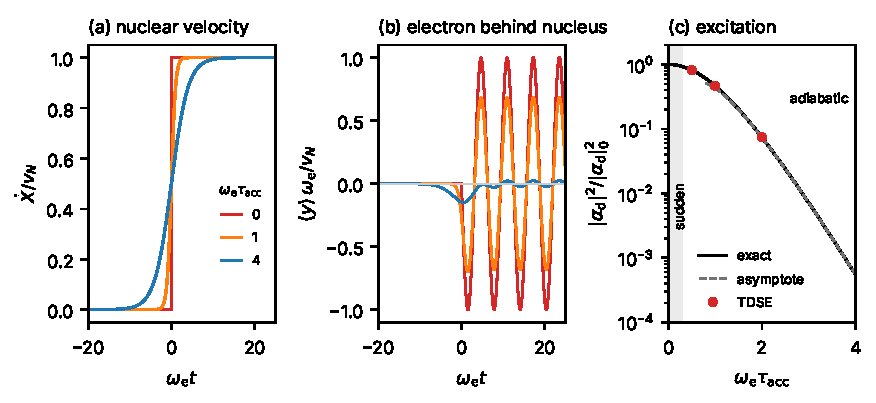
\includegraphics[width=\linewidth]{figures/ch06/fig6_1.pdf}
  \caption{Adiabatic and sudden responses of an electron to a moving nucleus, in a model in which one electron is bound to the nucleus by a harmonic force of frequency $\omega_{\mathrm{e}}$ and the nucleus follows a prescribed classical path. (a) The velocity of the nucleus, $\dot X = \tfrac12v_N[1 + \tanh(t/\tau_{\mathrm{acc}})]$, for acceleration times $\omega_{\mathrm{e}}\tau_{\mathrm{acc}} = 0$ (an instantaneous kick), 1 and 4. (b) The mean position $\langle y\rangle$ of the electron relative to the nucleus, in units of $v_N/\omega_{\mathrm{e}}$, for the same three cases. After a kick the electron oscillates about the nucleus with the full amplitude; after a slow acceleration it lags behind while the force acts and returns to rest. (c) The excitation $|\alpha_{\mathrm{d}}|^2 = -\ln P_0$, with $P_0$ the probability that the electron ends in the ground state, divided by its value $|\alpha_{\mathrm{d}}|^2_0 = m_ev_N^2/2\omega_{\mathrm{e}}$ for an instantaneous kick, against $\omega_{\mathrm{e}}\tau_{\mathrm{acc}}$. Solid: the exact result \cref{eq:6.1-model}. Dashed: its adiabatic asymptote $\pi^2(\omega_{\mathrm{e}}\tau_{\mathrm{acc}})^2\ee^{-\pi\omega_{\mathrm{e}}\tau_{\mathrm{acc}}}$. Dots: $-\ln P_0$ from a split-operator solution of the time-dependent Schr\"odinger equation for $m_ev_N^2/2\omega_{\mathrm{e}} = 1/2$. Shaded: the sudden region $\omega_{\mathrm{e}}\tau_{\mathrm{acc}} < 0.3$, where the excitation is within \SI{10}{\percent} of its sudden value.}
  \label{fig:6-sudden}
\end{figure}

For a nucleus in a crystal two times matter: how long the kick lasts, and how soon the neighbors start pulling the nucleus back. The kick itself is fast. A classical estimate of its duration, a heuristic only, is the time the dark matter takes to cross the region where it interacts with the nucleus. For a contact interaction and a silicon nucleus of radius \SI{3.5}{fm} this is $\SI{4e-21}{s}$ at $v_{\mathrm{max}}$, while $1/\Eg = \SI{0.56}{fs}$. The deceleration is slow. After the kick the nucleus is pulled back by the lattice over a time $\sim1/\omega_{\mathrm{ph}}$, which is the adiabatic regime for every excitation across the gap. In the model, take a nucleus that is kicked at $t = 0$ and then oscillates at $\omega_{\mathrm{ph}}$ in a harmonic well, $X(t) = (v_N/\omega_{\mathrm{ph}})\sin\omega_{\mathrm{ph}}t$ for $t > 0$. Its acceleration is $\ddot X = v_N\delta(t) - v_N\omega_{\mathrm{ph}}\sin(\omega_{\mathrm{ph}}t)\,\Theta(t)$, and $\int\dd t\,\ddot X\,\ee^{\ii\omega_{\mathrm{e}}t} = v_N/[1 - (\omega_{\mathrm{ph}}/\omega_{\mathrm{e}})^2]$, so $|\alpha_{\mathrm{d}}|^2$ exceeds the free-recoil value by the factor $[1 - (\omega_{\mathrm{ph}}/\omega_{\mathrm{e}})^2]^{-2}$. With $\omega_{\mathrm{ph}}/\omega_{\mathrm{e}}$ set to the ratio $\omega_{\mathrm{opt}}/\Eg = 0.055$ of the zone-center optical phonon of silicon, $\omega_{\mathrm{opt}} = \SI{64.1}{meV}$, to its gap, the factor is 1.006. A kicked nucleus in an insulator therefore excites its electrons as if it were free, with corrections of relative order $(\omega_{\mathrm{ph}}/\Delta E)^2$, the square of the small ratio that controls the adiabatic approximation. The sudden picture fails where that ratio is not small, for excitation energies comparable to phonon energies, as at the Fermi surface of a metal, and where the classical path itself fails, for recoil energies $q^2/2M$ that do not exceed a phonon energy (\cref{sec:5.6}). There the nucleus does not recoil, the kick creates a few phonons, and the electron--lattice response of \cref{sec:12.1} replaces the trajectory.

\subsection{The sudden kick}

In the sudden limit the result does not need perturbation theory. Immediately after the kick the electronic wavefunction is what it was before, $\Psi_0(r;u)$, but the nucleus moves with velocity $\vect{v}_N$. In the frame that moves with the nucleus, the electrons have all acquired the velocity $-\vect{v}_N$. A Galilean boost of every electron by $-\vect{v}_N$ multiplies the wavefunction by a plane wave:
\begin{equation}
  \Psi_0 \;\to\; \exp\Bigl(-\ii m_e\vect{v}_N\cdot\sum_e(\vect{r}_e - \vect{X})\Bigr)\Psi_0 , \qquad
  P_0 = \Bigl|\Bigl\langle\Psi_0\Bigr|\exp\Bigl(-\ii m_e\vect{v}_N\cdot\sum_e\vect{r}_e\Bigr)\Bigl|\Psi_0\Bigr\rangle\Bigr|^2 ,
  \label{eq:6.1-boost}
\end{equation}
where in $P_0$, the probability that the electrons are found in the ground state around the moving nucleus, the phase $\ee^{\ii m_e\vect{v}_N\cdot\vect{X}}$ drops out. This is Migdal's formulation~\cites{migdal1941ionization}[Eqs.~(1) and~(2)]{ibe2018migdal}. To first order in $v_N$ the amplitude of an excited state is $-\ii m_e\vect{v}_N\cdot\langle\Psi_j|\sum_e\vect{r}_e|\Psi_0\rangle$, a dipole transition driven by the kick. It agrees with \cref{eq:6.1-sudden1}. For an atom the adiabatic states depend on the nuclear position only through $\vect{r}_e - \vect{X}$, so that $\nabla_{\vect{X}}\Psi_0 = -\sum_e\nabla_e\Psi_0$, and the total electron momentum is $-\ii\sum_e\nabla_e = \ii m_e[H_{\mathrm{el}}, \sum_e\vect{r}_e]$. Taking the matrix element between $\Psi_j$ and $\Psi_0$, $\vect{d}_{j0} = m_e\Delta E_j\,\langle\Psi_j|\sum_e\vect{r}_e|\Psi_0\rangle$, and \cref{eq:6.1-sudden1} becomes the dipole amplitude. The derivative coupling of an atom is its dipole matrix element times the excitation energy and the electron mass.

For one electron in hydrogen the sudden result is exact. The Hamiltonian $p_e^2/2m_e + p_p^2/2m_p - \alpha/|\vect{r}_e - \vect{X}|$ separates into the motion of the center of mass $\vect{R}_{\mathrm{cm}} = (m_p\vect{X} + m_e\vect{r}_e)/M_{\mathrm{H}}$, with $M_{\mathrm{H}} = m_p + m_e$, and the relative coordinate $\vect{\rho} = \vect{r}_e - \vect{X}$, whose ground state is the 1s state with the reduced mass $\mu_{ep} = m_em_p/M_{\mathrm{H}}$ and the Bohr radius $a_{ep} = 1/(\alpha\mu_{ep})$. Dark matter that couples to the proton acts on the atom, to first order in its coupling, through $\ee^{\ii\vect{q}\cdot\vect{X}}$ (\cref{sec:2.2}); a coupling of the dark matter to the electron itself is a separate process, which we leave aside. Since $\vect{X} = \vect{R}_{\mathrm{cm}} - (m_e/M_{\mathrm{H}})\vect{\rho}$,
\begin{equation*}
  \ee^{\ii\vect{q}\cdot\vect{X}} = \ee^{\ii\vect{q}\cdot\vect{R}_{\mathrm{cm}}}\;\ee^{-\ii(m_e/M_{\mathrm{H}})\vect{q}\cdot\vect{\rho}} .
\end{equation*}
The first factor gives the whole atom the momentum $\vect{q}$. The second acts on the internal state like a momentum transfer $-(m_e/M_{\mathrm{H}})\vect{q}$ to the electron, and its ground-state expectation value is the elastic form factor \cref{eq:2.2-F1s} with $a_{ep}$ in place of $a_0$. Its argument is $(m_eq/M_{\mathrm{H}})\,a_{ep} = q/(\alpha m_p) = v_N/\alpha$, where $v_N = q/m_p$ is the velocity given to the proton, and the reduced-mass corrections cancel. With $a_0 = 1/(\alpha m_e)$ we may write the argument as $m_ev_Na_0$:
\begin{keyresult}[Sudden kick of a hydrogen atom]
A hydrogen atom in its ground state whose nucleus is given the velocity $v_N = q/m_p$ remains in its ground state with probability
\begin{equation}
  P_0 = \bigl|F_{1s}(m_ev_N)\bigr|^2 = \left[\frac{16}{(4 + v_N^2/\alpha^2)^2}\right]^2 \simeq 1 - \frac{v_N^2}{\alpha^2} \quad (v_N \ll \alpha) ,
  \label{eq:6.1-P0}
\end{equation}
and is excited or ionized with probability $1 - P_0$. The controlling ratio is that of the nuclear velocity to the orbital velocity $\alpha$ of the electron.
\end{keyresult}
The derivation used no assumption about time. In a first-order amplitude the momentum transfer is a single act, and the dark matter couples to the nuclear coordinate only. Nothing in a free atom decelerates the nucleus afterward, and the separation of the center of mass does the work that suddenness did in \cref{eq:6.1-boost}. Ibe et al.\ derive the general atom in this way, with the amplitude of every electronic transition given by \cref{eq:6.1-boost} and the energy of the atom conserved overall~\cite[Eqs.~(55)--(58)]{ibe2018migdal}. For more than one electron the separation is not exact, and the argument $m_ev_N$ is corrected at relative order $m_e/M$; \cref{sec:12.2} makes this precise.

The fraction $1 - P_0$ of nuclear recoils that leave the atom excited or ionized is the \emph{Migdal effect}. Its interest for dark-matter searches is the energy it adds. A recoil of a few hundred eV in silicon may be below the threshold of a phonon or charge readout. An electron--hole pair from the same event, carrying at least the gap, is easy to count. In a crystal the electrons are shared between atoms, and the excitation is an electron--hole pair rather than an atomic transition.

\begin{workedexample}{Ground-state survival of a kicked hydrogen atom}\label{we:6-hydrogen}
Dark matter of $\mchi = \SI{1}{GeV}$ scatters elastically off a hydrogen atom at rest, at the largest laboratory speed $v_{\mathrm{max}} = 2.650\times10^{-3}$ (\cref{eq:1.2-vmax}). The atom has the mass $M_{\mathrm{H}} = \SI{938.783}{MeV}$, the reduced mass is $\mu_{\chi\mathrm{H}} = (1000 \times 938.783/1938.783)\,\si{MeV} = \SI{484.2}{MeV}$, and the largest momentum transfer is $q = 2\mu_{\chi\mathrm{H}}v_{\mathrm{max}} = \SI{2.566}{MeV}$, at which the atom recoils with $q^2/2M_{\mathrm{H}} = \SI{3.51}{keV}$.

The proton, of mass $m_p = \SI{938.272}{MeV}$, is kicked to $v_N = q/m_p = 2.735\times10^{-3}$, or \SI{820}{km.s^{-1}}; dark matter as heavy as the target bounces it at about its own speed. In units of the orbital velocity, $v_N/\alpha = 0.375$. Then $F_{1s}(m_ev_N) = 16/(4 + 0.1405)^2 = 0.933$, and \cref{eq:6.1-P0} gives
\begin{equation*}
  P_0 = 0.871 , \qquad 1 - P_0 = 0.129 .
\end{equation*}
One such recoil in eight leaves the atom excited or ionized, with at least the \SI{10.2}{eV} of the $1s \to 2p$ transition in its electrons. The small-$v_N$ form, $v_N^2/\alpha^2 = 0.140$, is \SI{9}{\percent} high at this velocity. The atom survives with probability one half at $v_N/\alpha = 0.87$, where $F_{1s}^2 = \tfrac12$ (\cref{we:2-hydrogen}): $v_N = 6.35\times10^{-3}$, $q = \SI{5.96}{MeV}$ and a recoil of \SI{18.9}{keV}, beyond the reach of dark matter at this mass.

Is the kick sudden? The excitation energies start at $\Delta E = \tfrac38\alpha^2m_e = \SI{10.2}{eV}$, so the electron responds on the time $1/\Delta E = \SI{0.065}{fs}$. Dark matter with a contact interaction crosses the proton, of charge radius \SI{0.84}{fm}~\cite{mohr2025codata}, in $\SI{1.1e-21}{s}$, and $\Delta E\,\tau_{\mathrm{acc}} = 1.6\times10^{-5}$: on the scale of \cref{fig:6-sudden}(c) the kick is instantaneous.

For the kick of the opening, $v_N = 1.95\times10^{-4}$ for a silicon nucleus, the same formula gives $1 - P_0 = 7.1\times10^{-4}$ for an electron bound as in hydrogen. The outer electrons of silicon are bound more weakly and the inner ones far more strongly, so this is an order-of-magnitude statement.
\end{workedexample}
